\documentclass[10pt,conference]{IEEEtran}

\usepackage{amssymb,amsmath}
\usepackage[T1]{fontenc}
\usepackage{ifpdf}
\usepackage{url}

\usepackage[pdftex]{graphicx}
\graphicspath{{figs/}}
\DeclareGraphicsExtensions{.png,.jpg, .pdf}

\usepackage{float}
%\usepackage[caption=false,font=footnotesize]{subfig}
\usepackage[font=footnotesize]{caption}
\usepackage{subcaption}
\usepackage{setspace}
\usepackage{balance}
\pdfminorversion=6
\hyphenation{op-tical net-works semi-conduc-tor}
\newcommand{\indentitem}{\setlength\itemindent{0pt}}
\usepackage{algorithmic}
\usepackage{algorithm}
\newcommand{\algorithmicinput}{\textbf{Input:}}
\newcommand{\INPUT}{\item[\algorithmicinput]}
\newcommand{\algorithmicoutput}{\textbf{Output:}}
\newcommand{\OUTPUT}{\item[\algorithmicoutput]}
\renewcommand{\algorithmicrequire}{\textbf{Pre Condition:}}
\renewcommand{\algorithmicensure}{\textbf{Post Condition:}}
\floatname{algorithm}{Procedure}
\usepackage{tikz}
\usetikzlibrary{matrix,arrows,circuits.ee,circuits.ee.IEC,shapes.geometric,shapes.misc}
\newcommand{\iap}{\textit{DREMS}}
\newcommand{\iapfull}{\textbf{D}istributed \textbf{RE}altime \textbf{M}anaged \textbf{S}ystem}% Algorithmic modifications
\newcommand{\ALOOP}[1]{\ALC@it\algorithmicloop\ #1%
  \begin{ALC@loop}}
\newcommand{\ENDALOOP}{\end{ALC@loop}\ALC@it\algorithmicendloop}
\renewcommand{\algorithmicrequire}{\textbf{Input:}}
\renewcommand{\algorithmicensure}{\textbf{Output:}}
\newcommand{\algorithmicbreak}{\textbf{break}}
\newcommand{\BREAK}{\STATE \algorithmicbreak}
\newenvironment{noindlist}
 {\begin{list}{\labelitemi}{\leftmargin=0.1em \itemindent=0em \itemsep=0.3em}}
 {\end{list}}
\usepackage{multirow}

\usepackage{hyperref}

\begin{document}
\title{Experimental Validation of Timing Analysis for Component-based Distributed Real-time Embedded Systems }
\vspace{-0.1in}
\author{\IEEEauthorblockN{Pranav Srinivas Kumar and Gabor Karsai} 
	\IEEEauthorblockA{
		Institute for Software-Integrated Systems\\
		Department of Electrical Engineering and Computer Science\\
		Vanderbilt University, Nashville, TN 37235, USA \\
		Email:\{pkumar, gabor\}@isis.vanderbilt.edu
	}
}

% make the title area
 
\setcounter{page}{1}
\maketitle

\begin{abstract}
%Architecture-oriented domain-specific modeling languages (DSML) can provide a concise and modular abstraction for the structural and behavioral properties of a component-based system. DSMLs are increasingly used in distributed real-time (DRE) systems to manage the complexity and heterogeneity of architectural specifications, both in software and hardware. Such languages also enable model transformations, development automation and design-time analysis before deployment. 

This paper presents a timing analysis approach for modeling and verifying component-based software applications hosted on distributed real-time embedded (DRE) systems. Although schedulability analysis for real-time systems has been a considerably well-studied field, various general-purpose timing analysis tools are not intuitively applicable to all system designs, especially when domain-specific properties such as hierarchical scheduling schemes, time-varying networks and component-based interaction patterns directly influence the temporal behavior. Thus, there is still a need to develop analysis tools that are tightly coupled with the target system paradigm and platform while being generic and extensible enough to be easily modified for a range of systems. In this context, we have developed a Colored Petri Net-based schedulability analysis tool that integrates with a domain-specific modeling language and component model and that simulates and verifies temporal behavior for component operations in mission-critical DRE systems. Our results show the scalable utility of this approach for preemptive and non-preemptive hierarchical scheduling schemes in distributed scenarios.
\end{abstract}

\begin{IEEEkeywords}
	component-based, real-time, distributed, colored petri nets, 
	timing, schedulability, analysis
\end{IEEEkeywords}
\section{Introduction}

Real-time systems, by definition, must meet operational deadlines. These deadlines constrain the amount of time permitted to elapse between a stimulus provided to the system and a response generated by the system. Delayed responses or missed task deadlines can have catastrophic effects on the function of the system, especially in the case of safety- and mission-critical applications. This is the primary motivation for design-time schedulability analysis and verification of systems. 

There is a wealth of existing literature studying real-time task scheduling theory and timing analysis in uniprocessor and multiprocessor systems \cite{Audsley1995, Sha2004}. There are also several modeling, schedulability analysis and simulation tools \cite{MAST1, Cheddar, TIMES, PTIDES} that address various challenges in verifying real-time requirements although many such tools are appropriate only for certain task models, interaction patterns, scheduling schemes, or analysis goals. For component-based architectures, model-based system designs are usually expressed in a formal domain such as timed automata \cite{Alur1994, Macariu2010}, controller automata \cite{Zhang2012}, high-level Petri nets \cite{masri2009} etc. so that existing analysis tools such as UPPAAL \cite{UPPAAL} or CPN Tools \cite{CPNTools} can be used to verify either the entire system or its compositional parts. But, it is also evident that many of the existing schedulability analysis tools, though grounded in theory are not directly applicable to all system designs, especially with respect to domain-specific properties such as component interaction patterns, distributed deployment, time-varying communication networks etc. 

To be useful, the analysis tools need to be tightly integrated with the target domain: the concurrency model used by the system. The classic thread-based concurrency model (with generic synchronization primitives) is too low-level and too generic, it is hard to use, and hard to analyze. For pragmatic reasons, more restrictive, yet useful concurrency models are needed for which dedicated analysis tools can be developed. Our previous efforts \cite{MoDeVVa} were directed at this challenge. The target domain for that study was the DREMS component model \cite{DREMS13Software} which is the foundation of a software infrastructure addressing challenges in the design, development, and deployment of component-based embedded software for distributed applications like flight software for fractionated spacecraft. The physical nature of such systems requires strict, accurate and pessimistic timing analysis at design-time to avoid catastrophic situations at run-time. DREMS is implemented as a design-time tool suite and a run-time software platform that is enhanced by a component (concurrency) model with well-defined execution and interaction semantics. The platform relies on a temporally partitioned task scheduling scheme, a non-preemptive component-level operations scheduler, support for various communication and interaction patterns; all deployed on a distributed hardware platform.

Our contributions in this paper target efficient modeling and analysis techniques of temporal behavior for component-based applications that form distributed real-time embedded systems, such as DREMS. 

\begin{enumerate}
	\item We present an approach for modeling  the 'business logic': the operational behavior of each component in an application. The model uses a sequence of timed steps that are executed in the course of a component operation, including steps that specify interactions with other components. This approach enables abstracting the details of the middleware, while representing the temporal behavior of the component business logic. 
	\item We also present improvements to the CPN-based modeling approach that enables better analysis performance and scalability. These rely on heuristics that manage time variables and state space data structures more efficiently. 
	\item We also present advanced state space analysis methods and tools applied on the modeled system to reduce analysis time on medium to large-scale systems.
\end{enumerate}

The rest of this paper is organized as follows. Section \ref{sec:Related_Research} presents related research, reviewing and comparing existing analysis tools and formal methods. Sections \ref{sec:Target_System_Architecture} briefly describes the DREMS architecture, specifically the concepts of interest that are covered by the timing analysis tool. Section \ref{sec:Modeling} describes the business logic modeling approach to capture the operational behavior of components in the application. Section \ref{sec:Analysis} describes the analysis improvements we were able to achieve with structural changes to the analysis model. This section also briefly describes the application of advanced state space analysis methods that enable efficient state space searches while reducing the state space size and overall memory consumption. Section \ref{sec:Future_Work} evaluates possible extensions to this work before concluding with Section \ref{sec:Conclusions}.
\section{Related Research}
\label{sec:Related_Research}

% MAST
Verification of component-based systems requires significant amount of information about the application assembly, interaction semantics, and real-time properties. This information is primarily derived from the design model although many real-time metrics are not explicitly modeled. Using model descriptors, \cite{Lopez2006} describes interaction semantics and real-time properties of components. Using the MAST modeling and analysis framework \cite{MAST1, MAST2}, schedulability analysis and priority assignment automation is supported. Event-driven models are separated into several \emph{views} which are similar to hierarchical pages in some modeling formalisms, like Colored Petri Nets (CPN). Analysis efforts include the calculation of response times, blocking times, and slack times. %For every real-time application, a separate and independent real-time analysis model is generated for each mode of operation and analyzed

High-level Petri nets are a powerful modeling formalism for concurrent systems and have been integrated into many modeling tool suites for design-time verification. General-purpose Architecture Analysis \& Design Language (AADL) models have been translated into symmetric nets for qualitative analysis \cite{kordon_sn} and Timed Petri nets \cite{kordon2009} to check real-time properties such as deadline misses, buffer overflows etc. Similar to \cite{kordon2009}, our CPN-based analysis also uses bounded observer places \cite{Alpern1989} that observe the system behavior for property violations and prompt completion of operations. However, \cite{kordon2009} only considers periodic threads in systems that are not preemptive. Our analysis is aimed at a combination of preemptive and non-preemptive hierarchical scheduling with higher-level component interaction concepts. separately.

Several analysis approaches present tool-aided methodologies that exploit the capabilities of existing analysis and verification techniques. In the verification of timing requirements for composed systems, \cite{medina2011} uses the OMG UML Profile for Modeling and Analysis of Real-Time and Embedded Systems (MARTE) modeling standard and converts high-level design into MAST output models for concrete schedulability analysis. In a similar effort, AADL models are translated into real-time process algebra \cite{sokolsky2006} reducing schedulability analysis into a deadlock detection problem searching through state spaces and providing failure scenarios as counterexamples. Symbolic schedulability analysis has been performed by translating the task sets into a network timed automata, describing task arrival patterns and various scheduling policies. TIMES \cite{TIMES} calculates worst-case response times and scheduling policies by verifying timed automata with UPPAAL \cite{UPPAAL} model checking.

In order to analyze hierarchical component-based systems, the real-time resource requirements of higher-level components need to be abstracted into a form that enables scalable schedulability analysis. The authors in \cite{easwaran2006} present an algorithm where component interfaces abstract the minimum resource requirements of the underlying components, in the form of periodic resource models. Using a single composed interface for the entire system, the component at the higher level selects a value for operational period that minimizes the resource demands of the system. Such refinement is geared towards minimum waste of system resources.

\section{Component Execution Semantics}
\label{sec:ROSMOD}

A \emph{component operation} is an abstraction for the different tasks undertaken by a component. These tasks are implemented by the component's executor code written by the developer. Application developers provide the functional, \emph{business-logic} code that implements operations on the state variables e.g. a proportional-integral-derivative controller operation could receive the current state of dynamic variables from a \emph{Sensor} Component, and using the relevant gains, calculate a new state to which an \emph{Actuator} component should progress the system. In order to service interactions with the underlying framework and with other components, every component is associated with a \emph{message queue}. This queue holds instances of operations ('messages') that are ready for execution and need to be serviced by the component. These operations service either interaction requests (seen on communication ports) or service requests (from the underlying framework). An example for the latter is the use of component timers that can periodically (or sporadically) activate an operation. 

To facilitate component behavior that is free of deadlocks and race conditions, the component's execution is handled by a single thread. Operations in the message queue are therefore scheduled one at a time under a non-preemptive policy. A component dispatcher thread dequeues the next ready operation from the component message queue. This operation is scheduled for execution on a component executor thread. The operation is run to completion before another operation from the queue is serviced. This single-threaded execution helps avoid synchronization primitives such as internal state variables that lead to strenuous code development. Though components that share a processor still run concurrently, each component operation is executed by a single component-specific executor thread.

\begin{figure}[ht]
	\centering
	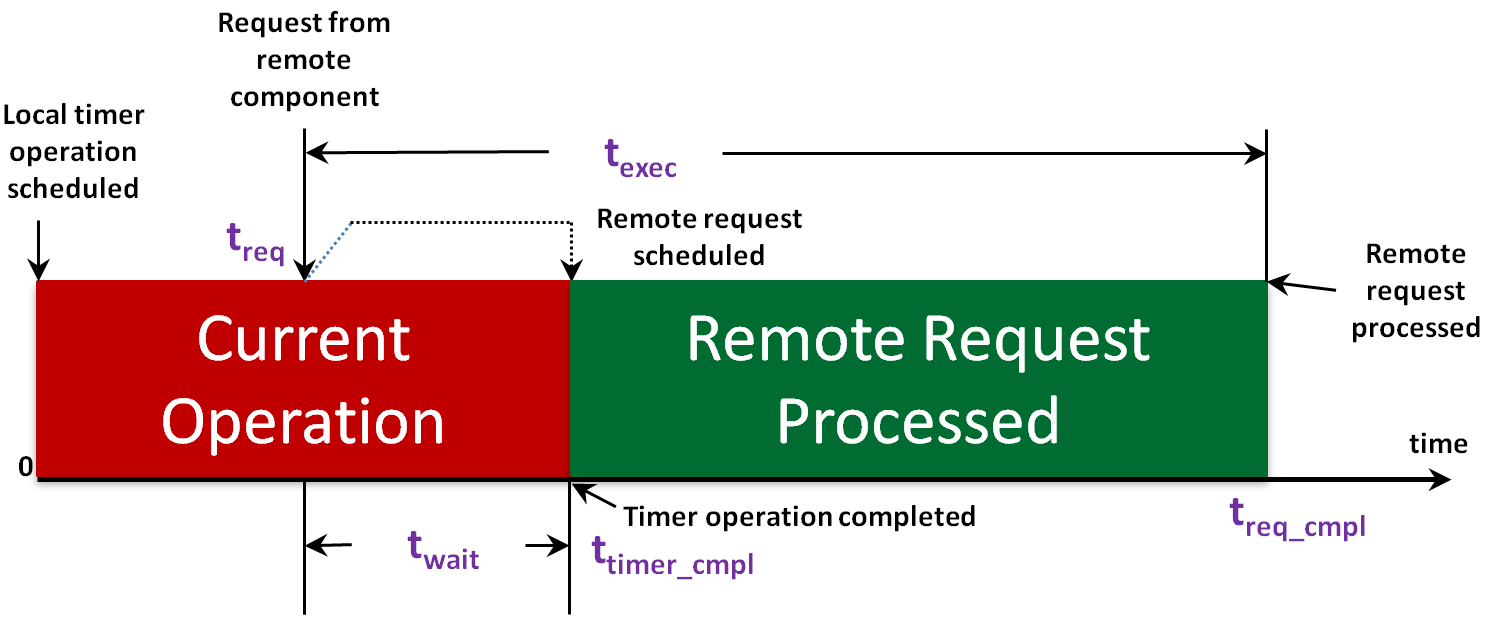
\includegraphics[width=0.5\textwidth]{cop_execution_semantics}
	\caption{Component Operation Execution Semantics: This figure shows the effects of the ROSMOD component scheduling on an incoming operation request. $t\_{req}$ represents the arrival time of a remote request. $t\_{wait}$ is the wait time of this request in the message queue while the current operation is still executing. $t\_{timer\_cmpl}$ is the time stamp at which the current operation completes executing. At this time, the remote request is finally scheduled for execution. $t\_{req\_cmpl}$ is the time stamp at which the remote request completes. The execution time, $t\_{exec}$ of this request is calculated as the difference in time stamps between $t\_{req\_cmpl}$ and $t\_{req}$.}
	\label{fig:cop_execution_semantics}
\end{figure}

Figure \ref{fig:cop_execution_semantics} shows the execution semantics of a component operation executed on a lone component executor thread. A simplifying assumption  to describe the semantics is that this component is the only component thread executing on this CPU. Assume that at $t=0$, this component is processing the expiry of a local timer. This operation is expected to complete at $t = t_{timer\_cmpl}$. However, at $t = t_{req}$, a service request is received from some remote component. Since the component operation scheduling is non-preemptive, regardless of the priority of this service, the request is not processed until $t_{timer\_cmpl}$. Therefore, the request is waiting in the message queue for $t_{wait} = t_{timer\_cmpl} - t_{req}$. At $t = t_{timer\_cmpl}$, the timer operation is marked as complete and the service request is processed. The total execution time of this service operation is calculated including the duration of the time for which this request waited in the component message queue i.e. $t_{exec} = t_{req\_cmpl} - t_{req}$. The wait times in the queue are further worsened when OS scheduling non-determinism is taken into account. There are specifically three ways in which the OS scheduling can delay operations: (1) if the application process is concurrently executing executor threads of multiple components of equal priority, then the threads are scheduled in Round-Robin fashion by the OS, (2) when mixed-criticality application processes are scheduled in tandem, the OS uses fixed-priority Round-Robin scheduling to schedule the process threads, and finally (3) temporally partitioned OS schedules further cause delays on component thread scheduling, which directly affects the scheduling and timely completion of component operations. 
\section{CPN Analysis Model}
\label{sec:CPN}

%\begin{figure}[h]
%	\centering
%	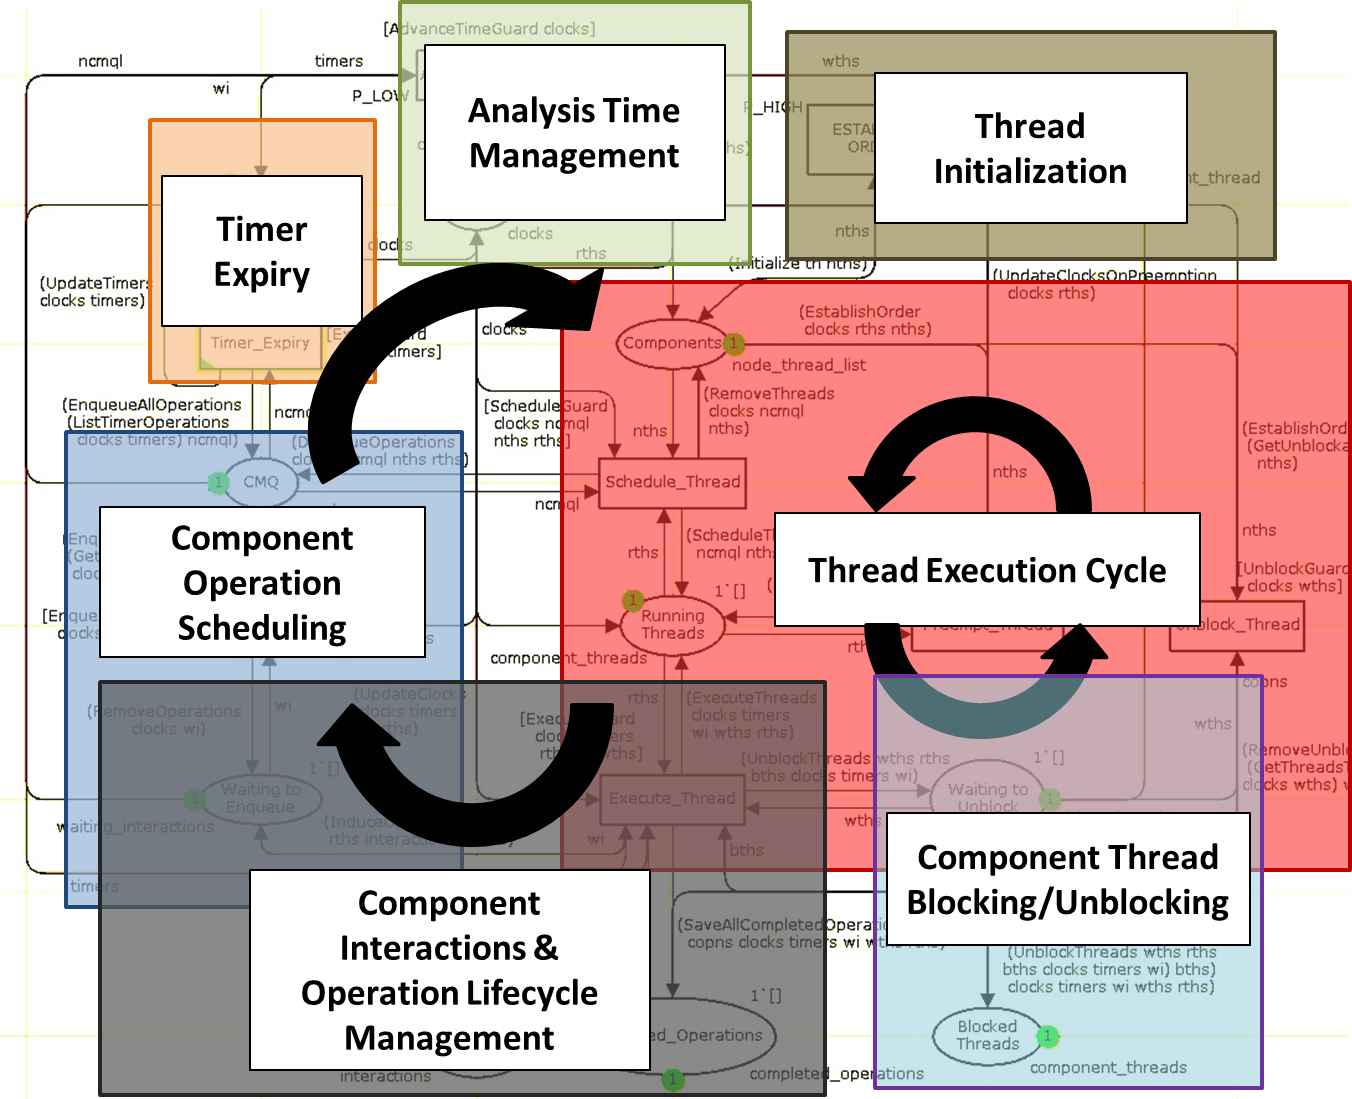
\includegraphics[width=0.4\textwidth]{hlcpn_structure}
%	\caption{Structural Aspects}
%	\label{fig:hlcpn_structure}
%\end{figure}

For the sake of brevity, a detailed description of both Colored Petri nets and our timing analysis model are not within the scope of this paper. The CPN analysis model consists of a collection of interacting sub-models, each responsible for modeling and simulating specific sub-systems in an application lifecycle e.g. thread scheduling, operation scheduling, thread execution, blocking and waiting times, timer expiries, and time progression. From the design model of the system, we generate the initial CPN tokens that are injected into places in this analysis model. Using the in-built state space analysis engine, we analyze the state space of the parameterized model to compute useful system properties \cite{kumar2014colored} \cite{SEUS} e.g. processor utilization, execution time plots, deadline violations etc.   





\section{Experimental Setup}
\label{sec:Testbed}

Cyber-Physical Systems require design-time testing and analysis before deployment. Several CPS scenarios require strict safety certification due to the mission-critical nature of the operation, e.g. flight control and automation. It is often times impossible to test control algorithms, fault tolerance procedures etc. on the real system due to both cost and hardware accessibility issues. To counter these issues, there are two principle methods in which a CPS can be tested and analyzed: (1) Construct a complete model of the CPS in a simulation environment e.g. Simulink \cite{Simulink} and simulate the system while accounting for run-time scenarios, (2) Establish a testing environment that can closely resemble the real CPS in both hardware and software. The problem with simulations is that it is hard to establish the network topology, emulate the application network and base processing power while running a physics simulation in the loop. Our RCPS testbed implements the latter alternative. The RCPS testbed consists of 32 BBB embedded boards running Linux. The gigabit ethernet port of each BBB is connected to a programmable OpenFlow \cite{openflow} enabled \emph{Communication Network} switch. Each RCPS node is also connected to a \emph{Physics Network} using a 10/100 USB-to-Ethernet adapter, since the BBBs only have one gigabit ethernet port. This network is connected to a \emph{Physics Simulation Machine} running cyber-physical systems simulations. For further details on the architecture of this testbed, readers are referred to our earlier work \cite{kumarTestbed}.

\if 0
\begin{figure}[h]
	\centering
	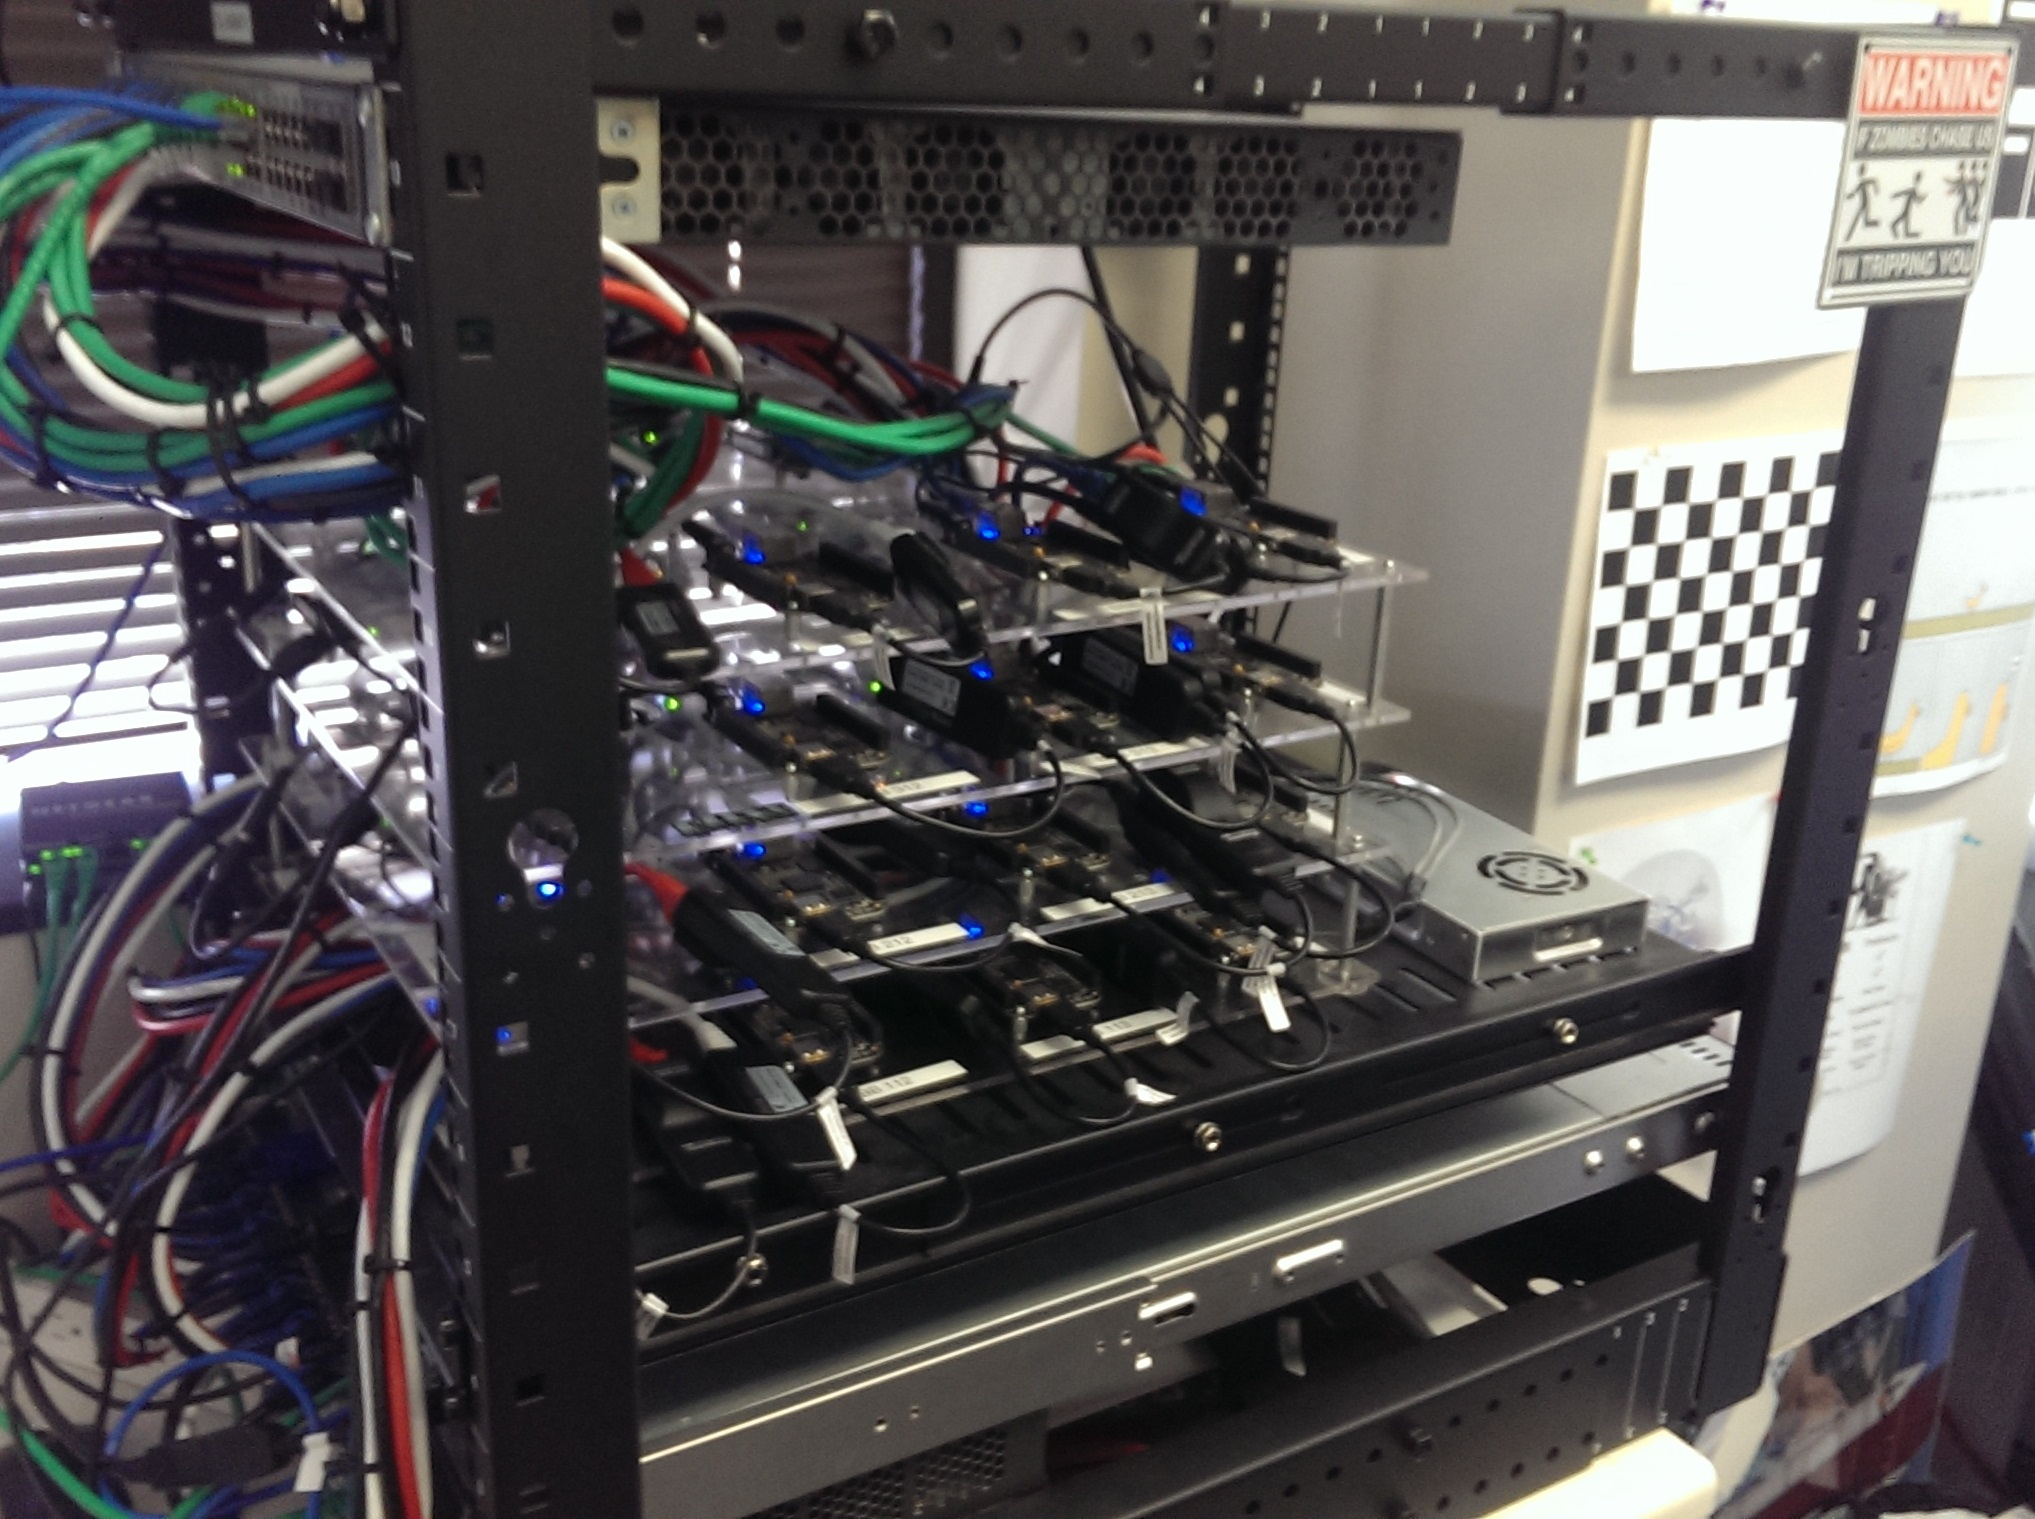
\includegraphics[width=0.45\textwidth]{testbed}
	\caption{RCPS Testbed}
	\label{fig:testbed}
\end{figure}
\fi

Using the RCPS testbed, a wide variety of DRE use-cases can be tested and accurately measured. This section briefly considers a few samples that test the various interaction patterns of ROSMOD, that are available to application developers and compares the measured results against the predicted worst-case execution time profiles of the modeled applications in our Colored Petri net-based analysis model. The expected result in all of these cases is to observe close but pessimistic behavior simulation from our analysis model i.e., the CPN analysis should be able to simulate and analyze the behaviors of the test cases and provide comparable and close approximations of the execution time plots while ensuring that the predicted \emph{worst-case execution times} (WCET), response times, processor utilization etc. are always conservative.
\section{Experimental Evaluation}
\label{sec:experiments}

Experimental validation should demonstrate that online measurements of the real-time system match with the timing analysis results in a way that the timing analysis results are always close but conservative. One of the biggest assumptions in our CPN work is the knowledge of worst-case execution times of the individual steps in the component operations. We have previously designed \cite{SEUS} a business-logic modeling grammar that captures the temporal behavior of component operations, especially WCET metrics for the different code blocks inside an operation. For example, consider a simple \emph{remote method invocation} (RMI) application as shown in Figure \ref{fig:rmi_application}. The client component is periodically triggered by an internal timer and executes a synchronous remote method invocation to a remote server component. The interaction here demands that the client component be blocked for the duration of time it takes the server to receive the operation, process its message queue, execute the relevant callback, and respond with output. 

Note that in Figure \ref{fig:rmi_application}, we only annotate isolated code blocks that take a fixed amount of execution time on a specific hardware architecture. These are the only measurements that we can reliably make with repeated testing and instrumentation. The client-side blocking delay is not measured because the number of factors responsible for this delay are numerous e.g. server's message queue state, scheduling non-determinism, network delays etc. In order to be able to predict this delay, we need to use state space analysis and search through the tree of possible executions to identify the worst-case blocking delay. This also means that our CPN model must capture and account for such delay-causing factors.
 

\begin{figure}[ht]
	\centering
	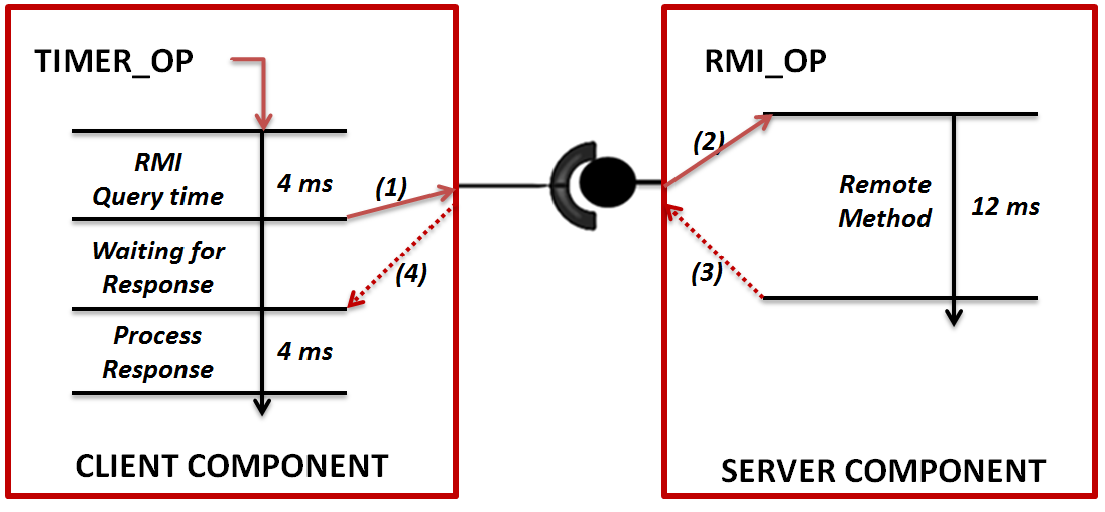
\includegraphics[width=0.4\textwidth]{rmi_application}
	\caption{RMI Application: A Periodically triggered client makes a remote method invocation to a server component. The assembly is annotated with estimated WCET on the different operational steps. The non-deterministic time here is the waiting time of the client, which is calculated using state space analysis.}
	\label{fig:rmi_application}
\end{figure}

WCET of component operational steps needs to be measured by having the component operation execute at real-time priority with no other component threads intervening this process. This measurement gives us a \emph{pure execution time} of the code block. The process must be repeated for all component operations to obtain meaningful worst-case estimates that are tailored to the target platform. Obtaining the WCET values by this method is not only more realistic but also an accurate representation of the target system. Once these individual numbers are obtained, the values are plugged into the CPN through our business-logic models. 

\begin{figure*}[h]
	\centering
	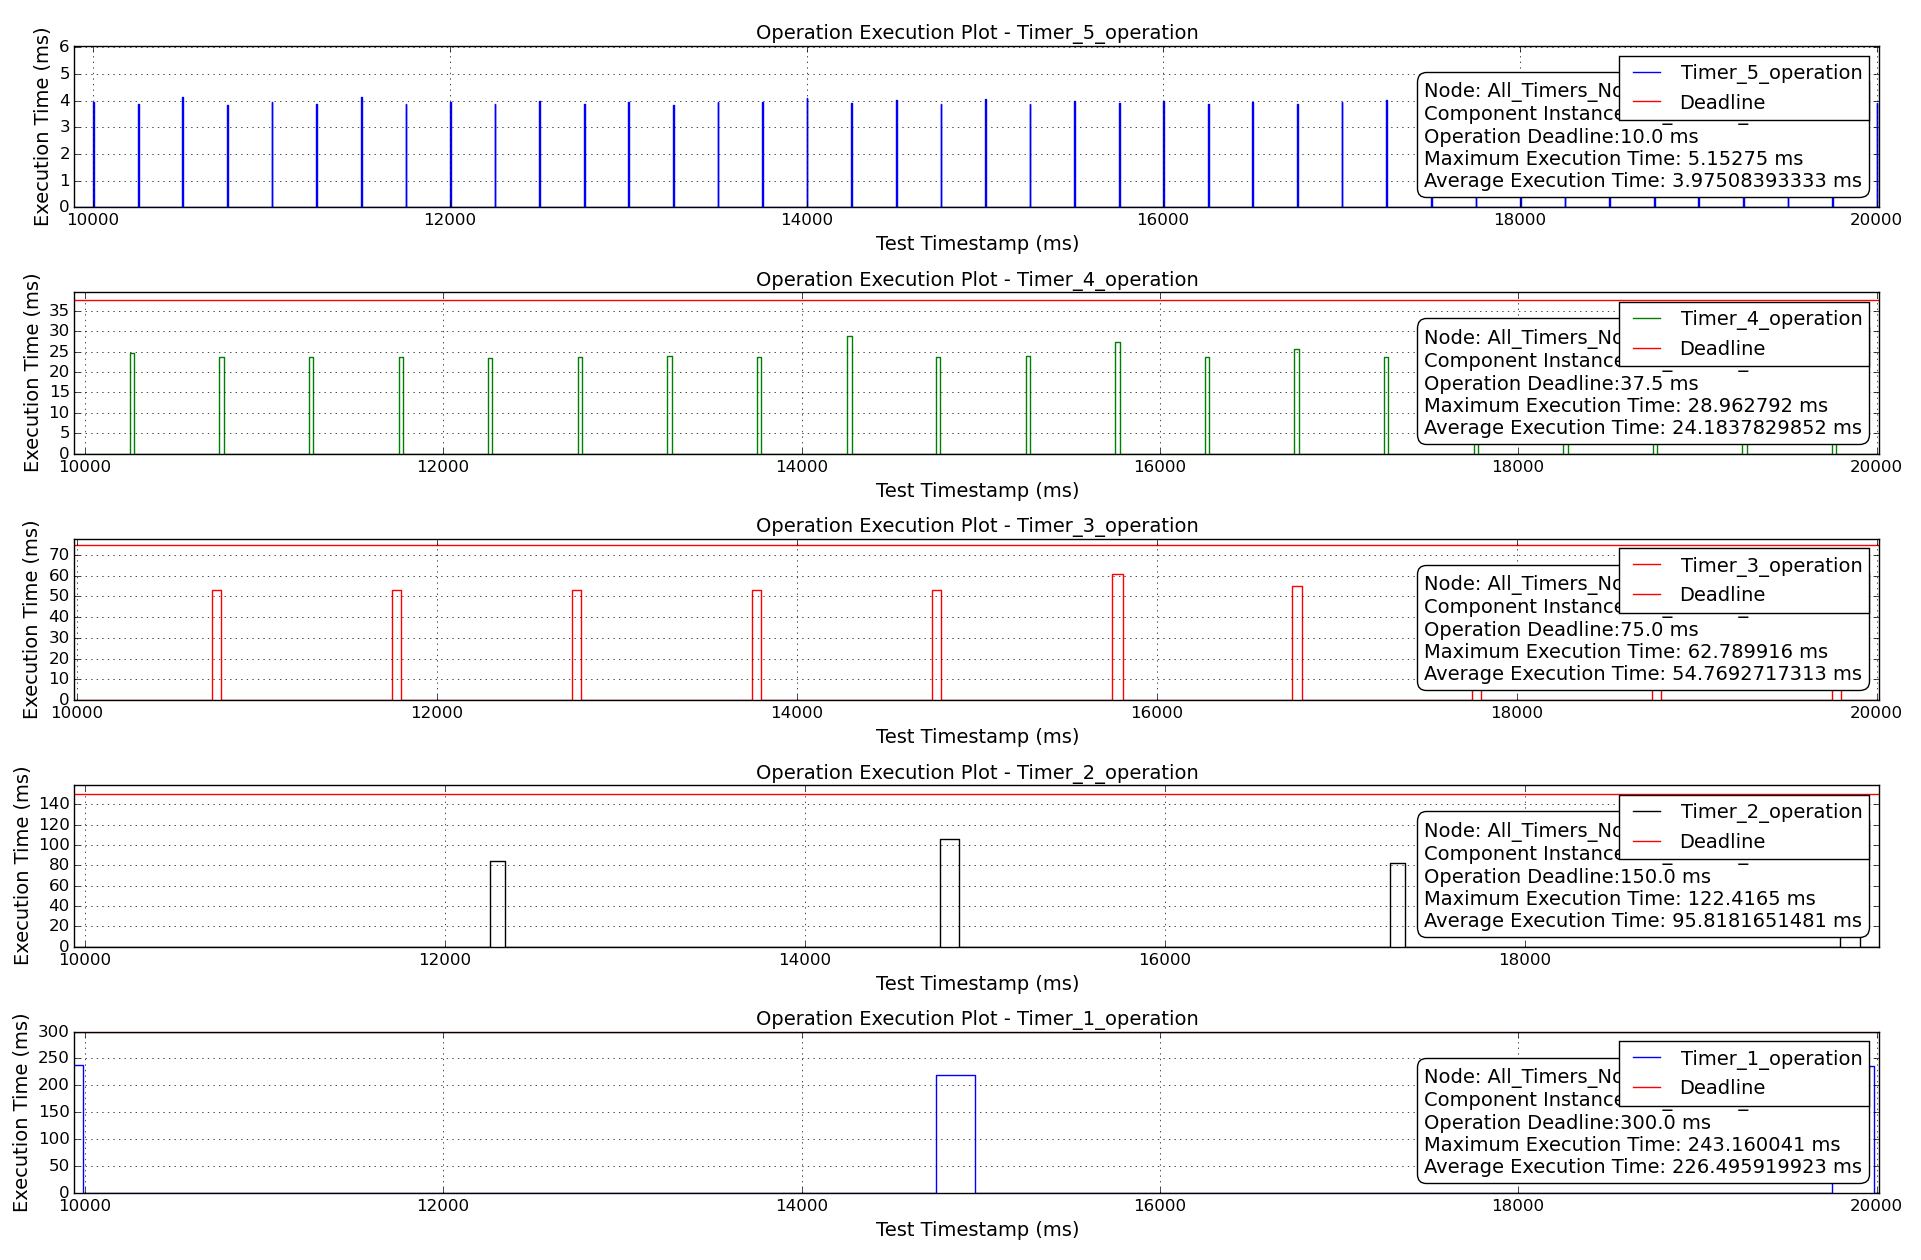
\includegraphics[width=\textwidth]{periodic-timers}
	\caption{Experimental Observation: Periodic Timers -- Five periodic timers with different frequencies and different priorities executed by a single component.}
	\label{fig:periodic-timers}
\end{figure*}

\begin{figure*}[h]
	\centering
	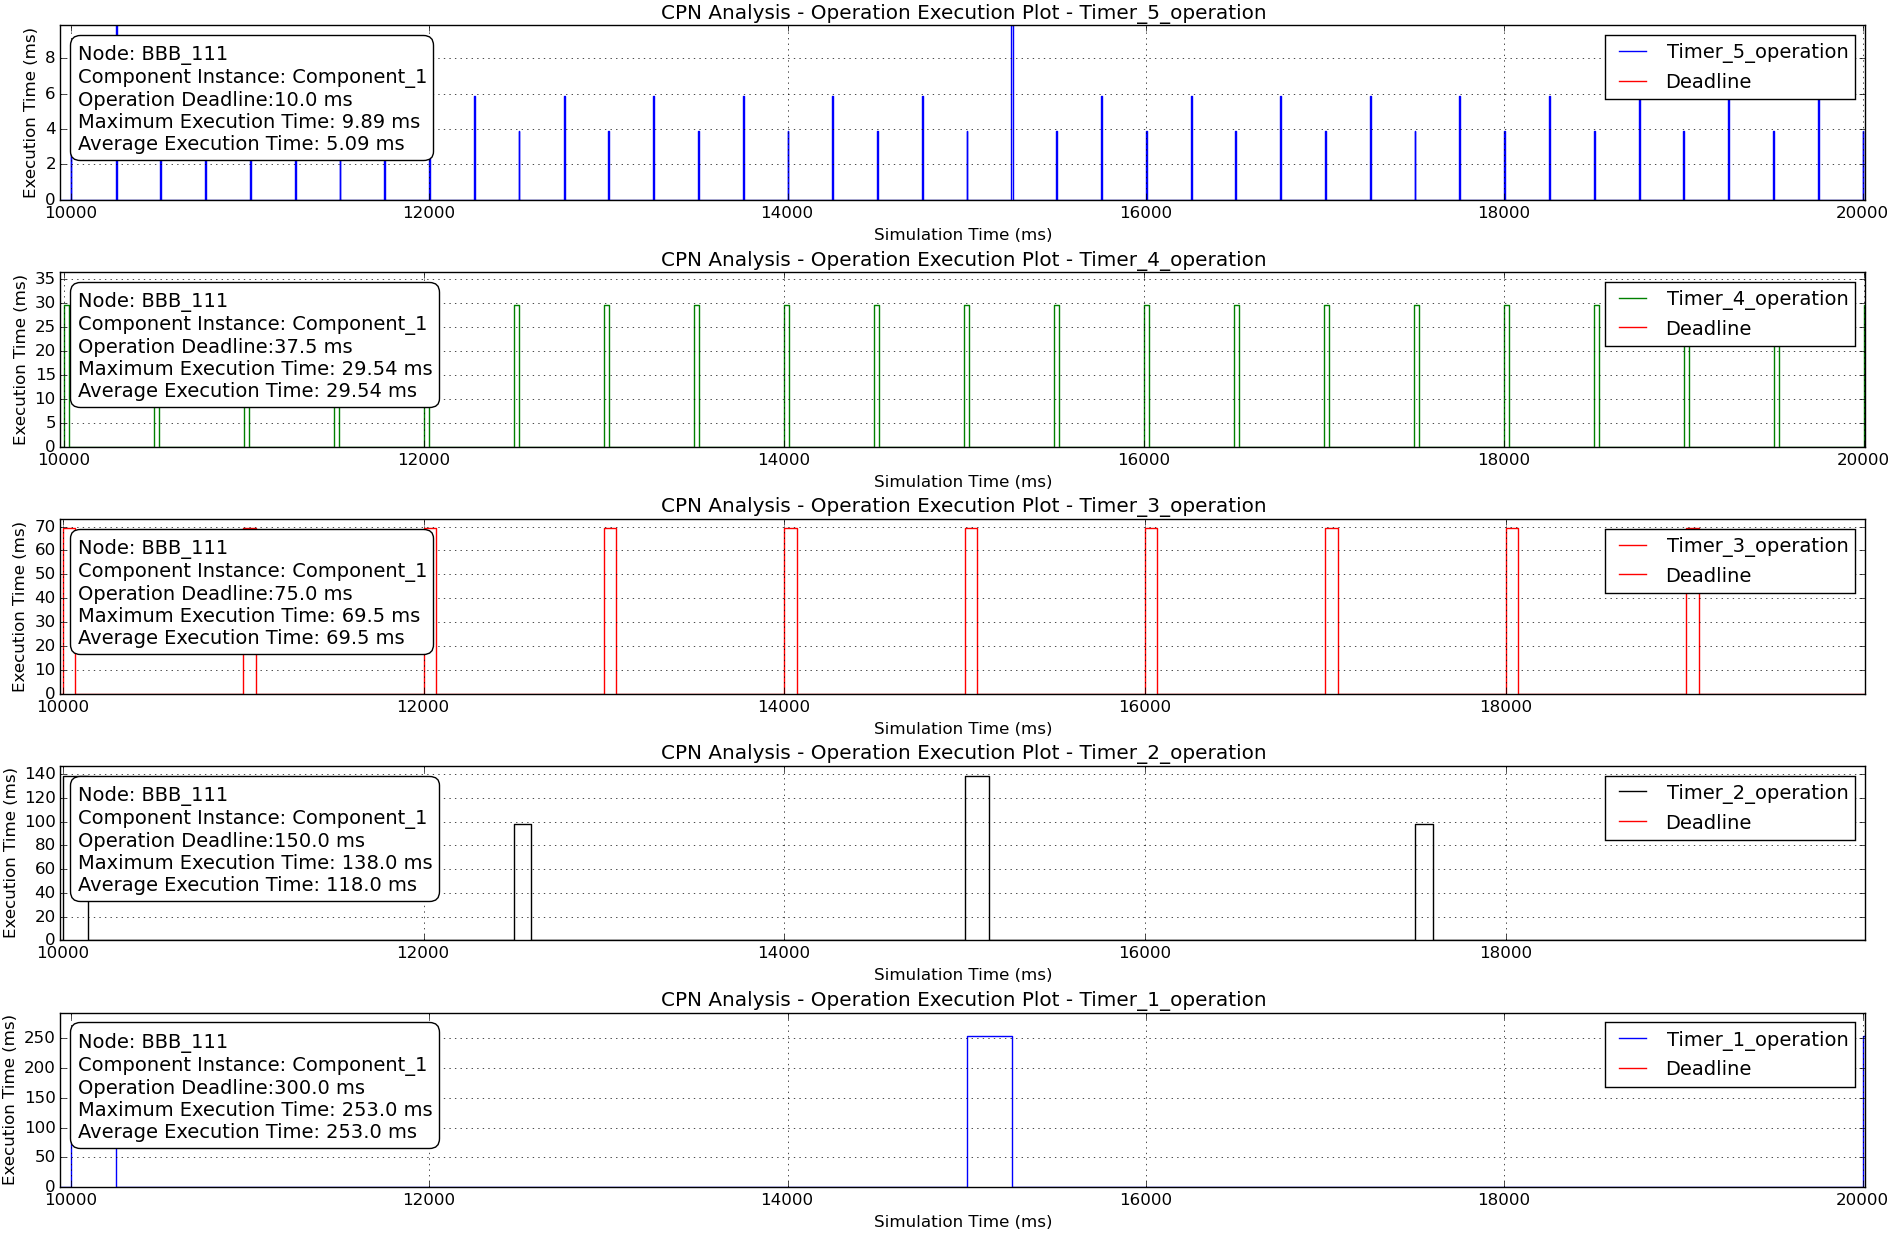
\includegraphics[width=\textwidth]{periodic-timers-cpn}
	\caption{CPN Analysis Results: Periodic Timers -- CPN state space analysis and estimation of WCET for five periodically triggered times contained by a single component. Execution time measurements for each timer is made separately and composed in the CPN model. The resultant analysis presents a conservative estimation on the WCET of the composed system.}
	\label{fig:periodic-timers-cpn}
\end{figure*}

%The remainder of this section presents some primitive interaction patterns and assemblies that have been evaluated. The presented results are restricted to some simple cases for thesake of brevity, though we have tested on medium-to-large scale examples spanning 25-30 computing nodes, and with up to a 100 components. The scalability of our model, however, is not within the scope of this paper as we have previously evaluated this metric \cite{SEUS}.

\if 0
\begin{figure*}[h]
	\centering
	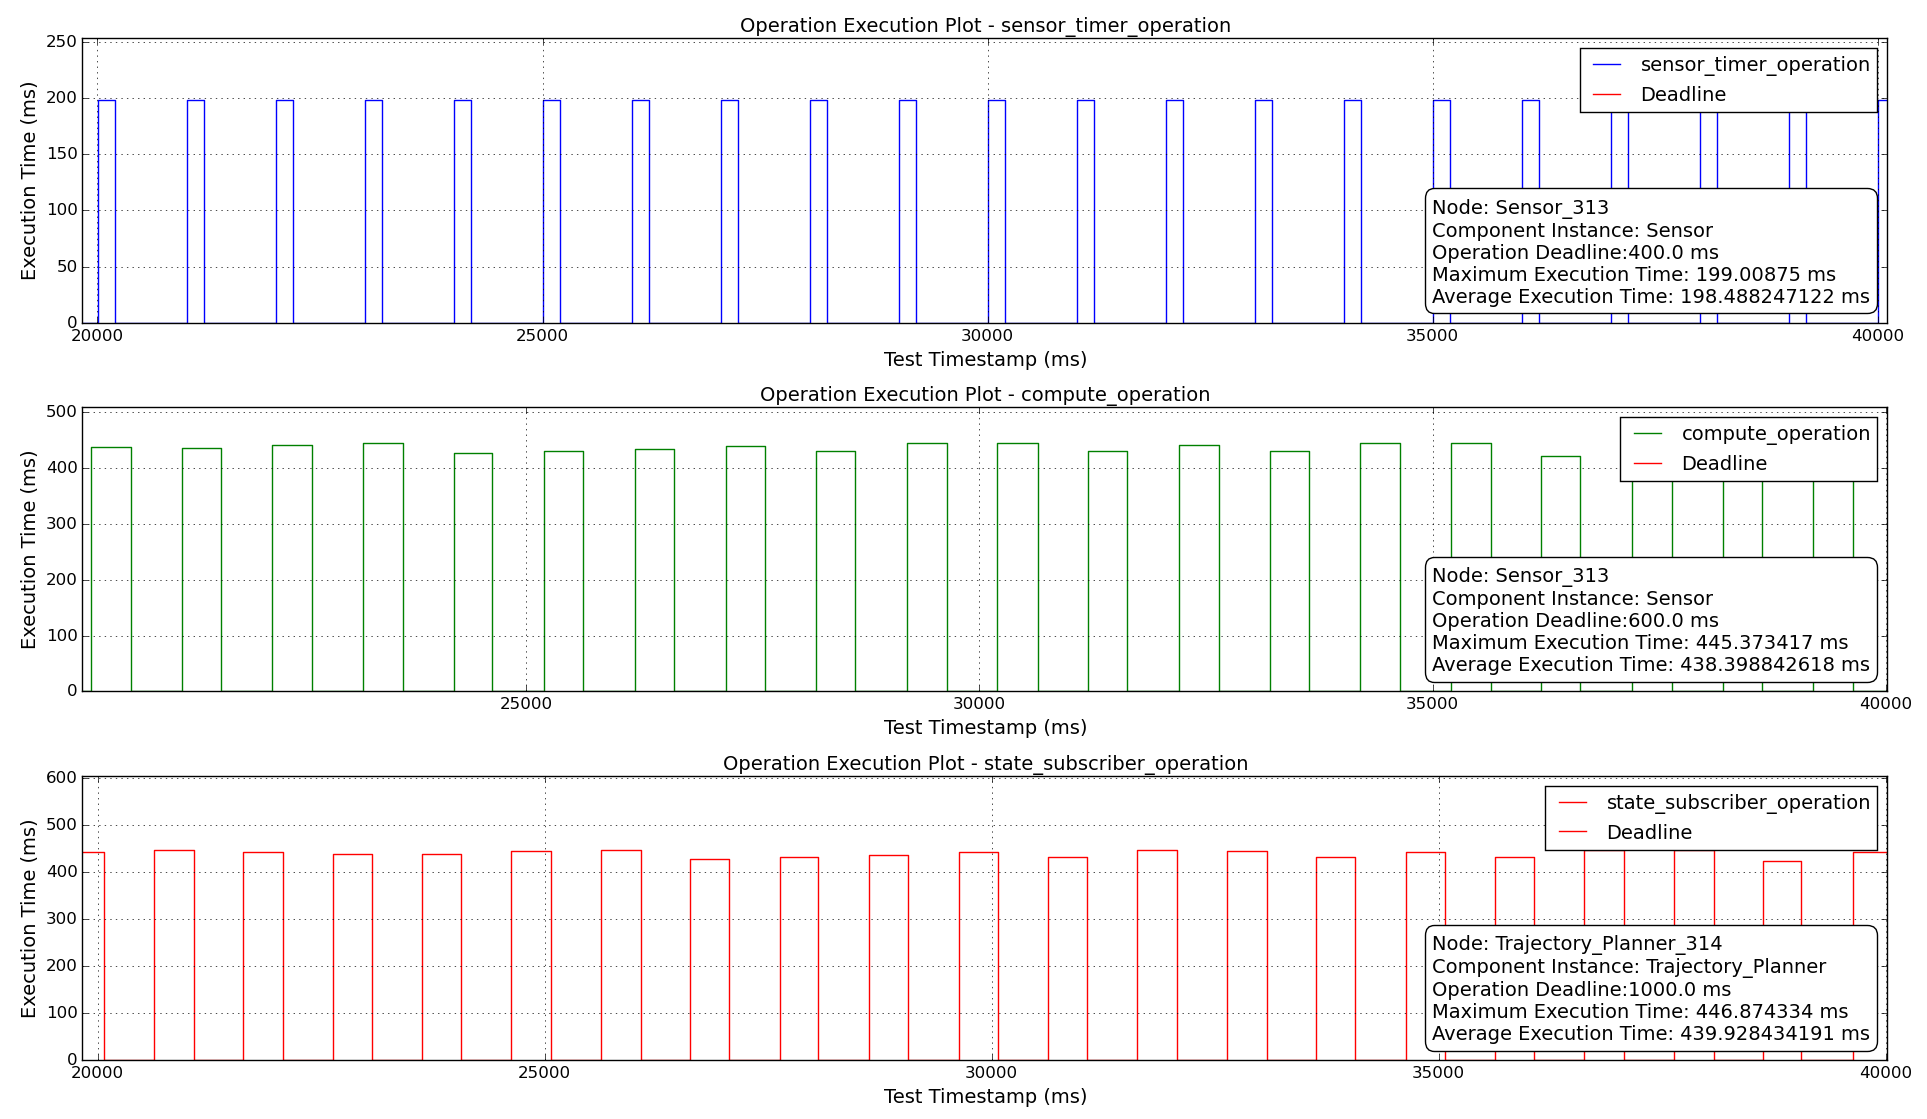
\includegraphics[width=0.75\textwidth]{trajectory-planner}
	\caption{Experimental Observation: Trajectory Planner}
	\label{fig:trajectory-planner}
\end{figure*}

\begin{figure*}
	\centering
	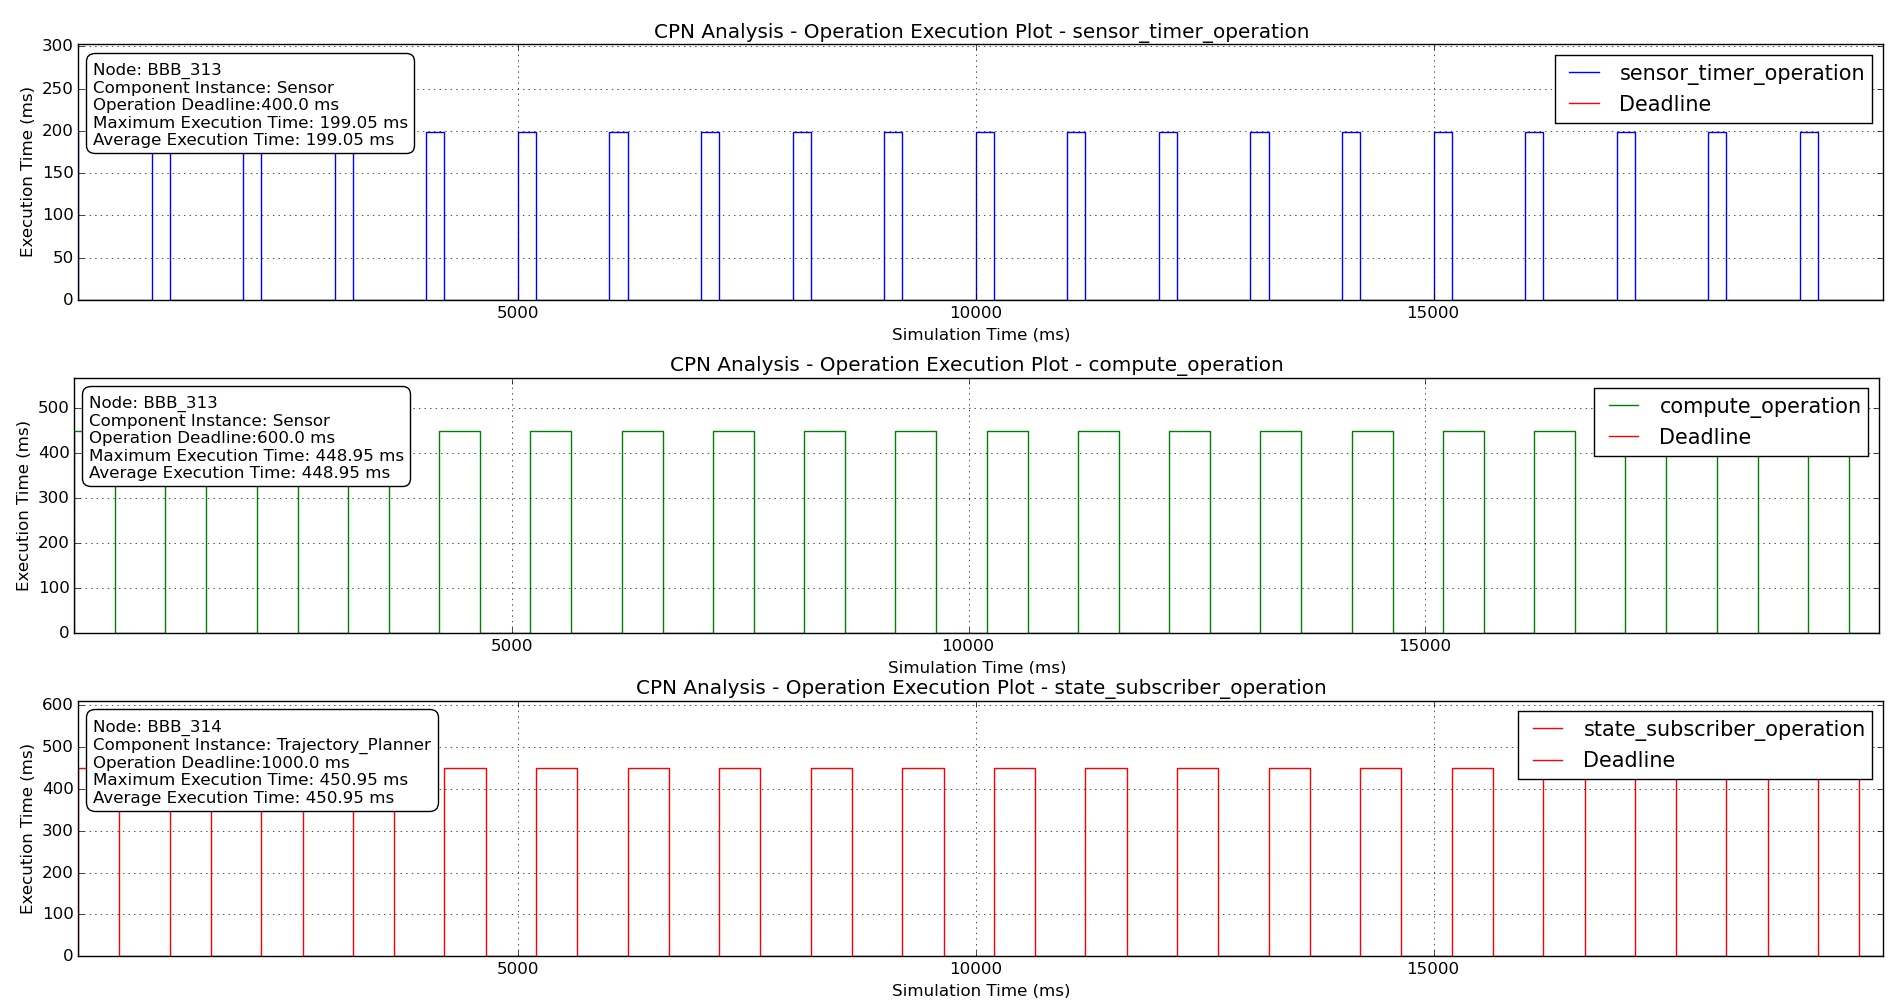
\includegraphics[width=0.75\textwidth]{trajectory-planner-cpn}
	\caption{CPN Analysis Results: Trajectory Planner}
	\label{fig:trajectory-planner-cpn}
\end{figure*}


\subsection{Trajectory Planner}

In the past \cite{kumar2014colored}, we have used a \emph{Trajectory Planner} deployment to illustrate the utility of our state space analysis. Figure \ref{fig:trajectory-planner} shows the execution time plot of this sample. A Sensor component is periodically triggered every second by the \emph{sensor\_timer} at which point it publishes a notification to the Trajectory Planner, alerting the planner of new sensor state. The planner component receives this notification on its \emph{state\_subscriber}. On receiving this message, the planner executes a remote method invocation to the \emph{compute} server located in the Sensor, blocked and waiting for a response. At this point, the \emph{compute\_operation} is executed on the Sensor which returns the updated sensor state. This unblocks the planner component which uses the new sensor state to perform trajectory planning tasks. 

This is a common interaction pattern in Cyber-Physical systems since embedded sensors are updated at a much higher frequency than a path planning entity. Thus, the planner can query the sensor at a lower rate to sample the sensor state. In this example, the planner is matching the frequency of the sensor since the execution cost is low. However, when more components are added to this deployment, the planner would have to fetch sensor state less frequently so as to not affect other system-level deadlines.  

\fi

\vspace{-0.05in}

\subsection{Time-triggered Operations}

Time-triggered operations are an integral part of our component model. ROSMOD components are dormant by default. A timer has to trigger a inactive component for all subsequent interactions to take place. Since the ROSMOD component model supports various scheduling schemes on a single component message queue, this following test evaluates a priority first-in first-out scheme. Multiple timers are created in a single component, each with a unique priority and period. A timer with a high frequency is assigned a high priority. Figure \ref{fig:periodic-timers} shows our experimental observations on a 5-timer example. 

Since ROSMOD components are associated with a single executor thread and component operations are non-preemptive, a low-priority operation could theoretically run forever, starving a higher priority operation from ever executing, leading to deadline violations e.g. \emph{Timer\_1\_operation} can affect all other higher priority timers. Figure \ref{fig:periodic-timers-cpn} shows our CPN prediction where such a scenario is evident. It can be seen that \emph{Timer\_5\_operation}, the timer with the highest priority is periodically seeing spikes in execution time, courtesy of other lower priority operations consuming CPU without preemption.

The analysis workflow, that has lead the results in Figure \ref{fig:periodic-timers-cpn}, is as follows: The time-triggered component is tested at real-time priority on the target platform, once for each timer which measures the pure execution time of each timer operation i.e. the time taken for each timer operation to execute on the target CPU without interruption. The WCET for each timer operation is then injected into our CPN analysis model and a composed timing analysis model is obtained. By performing bounded state space analysis, we derive the composed worst-case behavior of the component. Here, the execution times of each timer is affected by all other timers coupled with the execution semantics of the component model. These composed execution times will always be worse than the pure execution times due to factors like scheduling non-determinisms, context switching delays, and blocking behaviors. So, the results shown in Figure \ref{fig:periodic-timers-cpn} are the composed timing analysis results that can now be compared against the experimental observations in Figure \ref{fig:periodic-timers}. As evident in these figures, the CPN analysis results are conservative estimates of the real execution. 

%It must be noted here that the execution time values assigned to each timer operation in our CPN is the pure execution time i.e. the time taken for each timer operation to execute on the target CPU without interruption. This is the case for all operational execution times injected into the analysis model. If this is not done, then due to scheduling delays and interaction patterns, the CPN results will become gross overestimates. 

\begin{figure}[h]
	\centering
	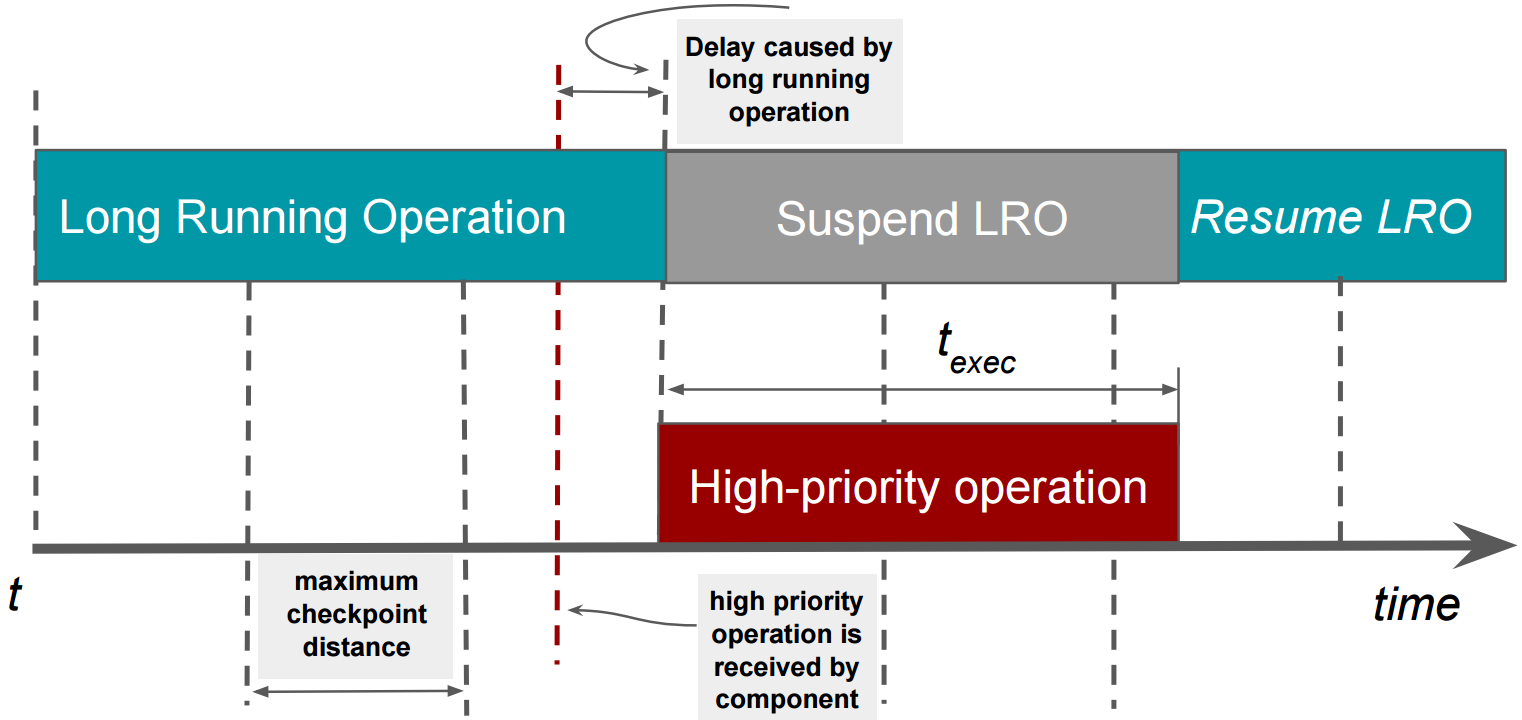
\includegraphics[width=0.5\textwidth]{lro-semantics}
	\caption{Long Running Operations (LRO) Timing Diagram -- The LRO is characterized by periodic checkpoints. At each checkpoint, the LRO checks to see if there are any higher priority operations waiting in the component message queue. If so, the LRO suspends till the higher priority operation completes and resumes and as soon as possible.}
	\label{fig:lro-semantics}
\end{figure}

\begin{figure}[h]
	\centering
	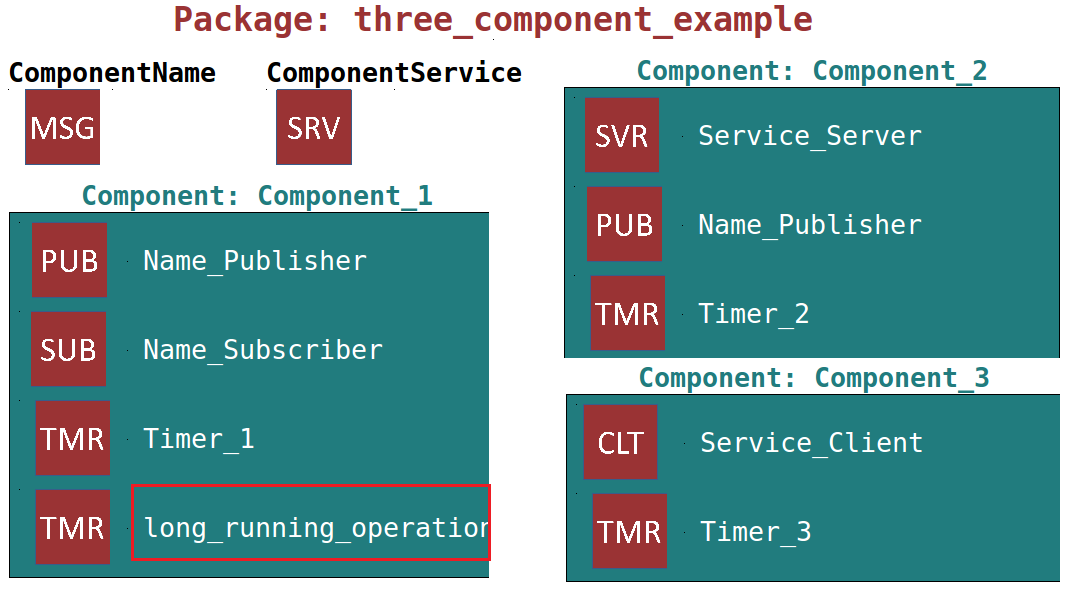
\includegraphics[width=0.4\textwidth]{three-components-lro-rosmod}
	\caption{Long Running Operation -- The Software Model consists of three components. Component\_1 contains a long running operation triggered by a sporadic timer.}
	\label{fig:three-components-lro-rosmod}
\end{figure}

\begin{figure*}[h]
	\centering
	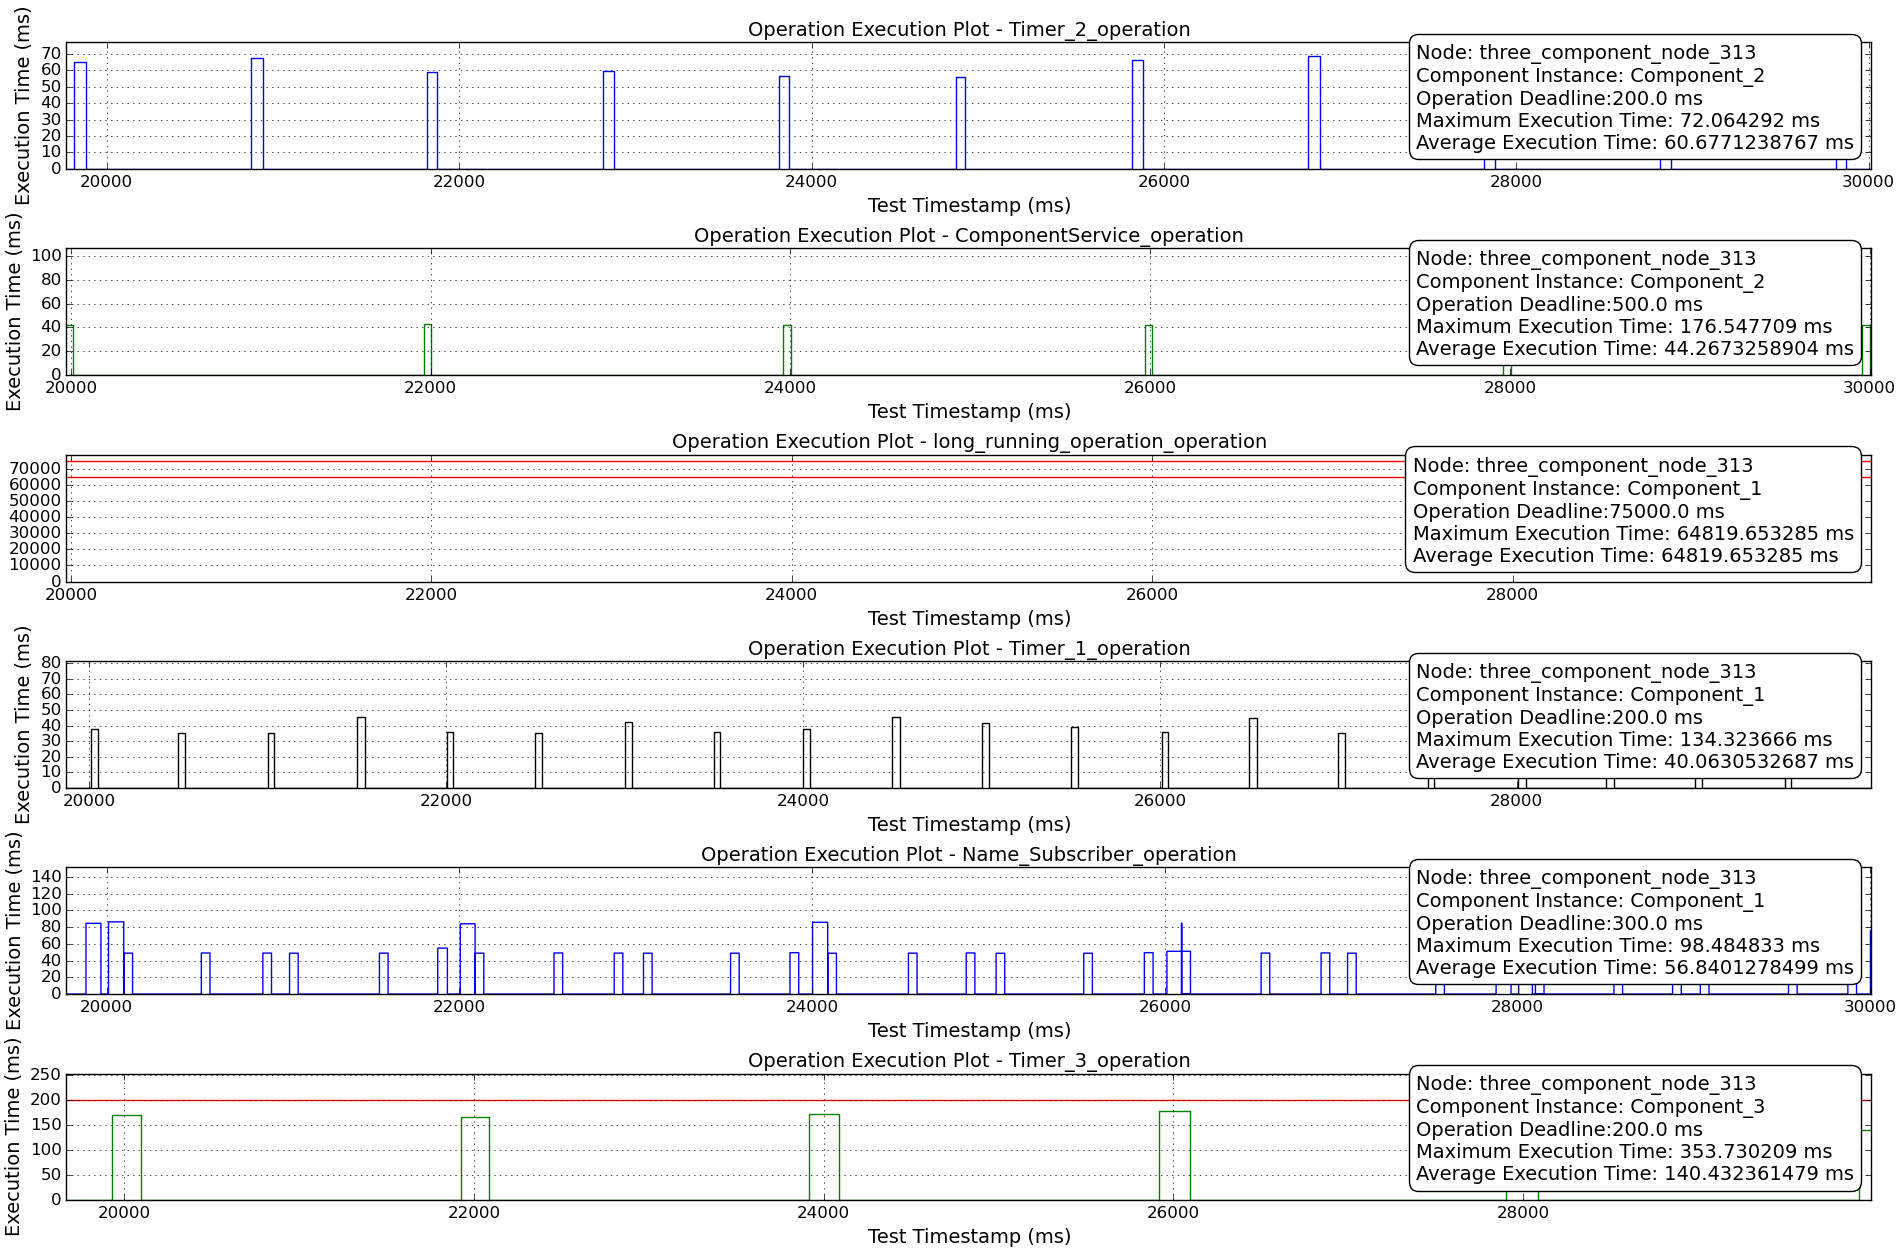
\includegraphics[width=\textwidth]{three-components-lro}
	\caption{Long Running Operations -- Experimental Observation. The goal of this test is to ensure that the long-running operation can execute concurrently in other time-triggered operations in Component\_1 and does not affect any timing properties. Periods and deadlines are chosen based on average-case performance.}
	\label{fig:three-components-lro}
\end{figure*}

\begin{figure*}[h]
	\centering
	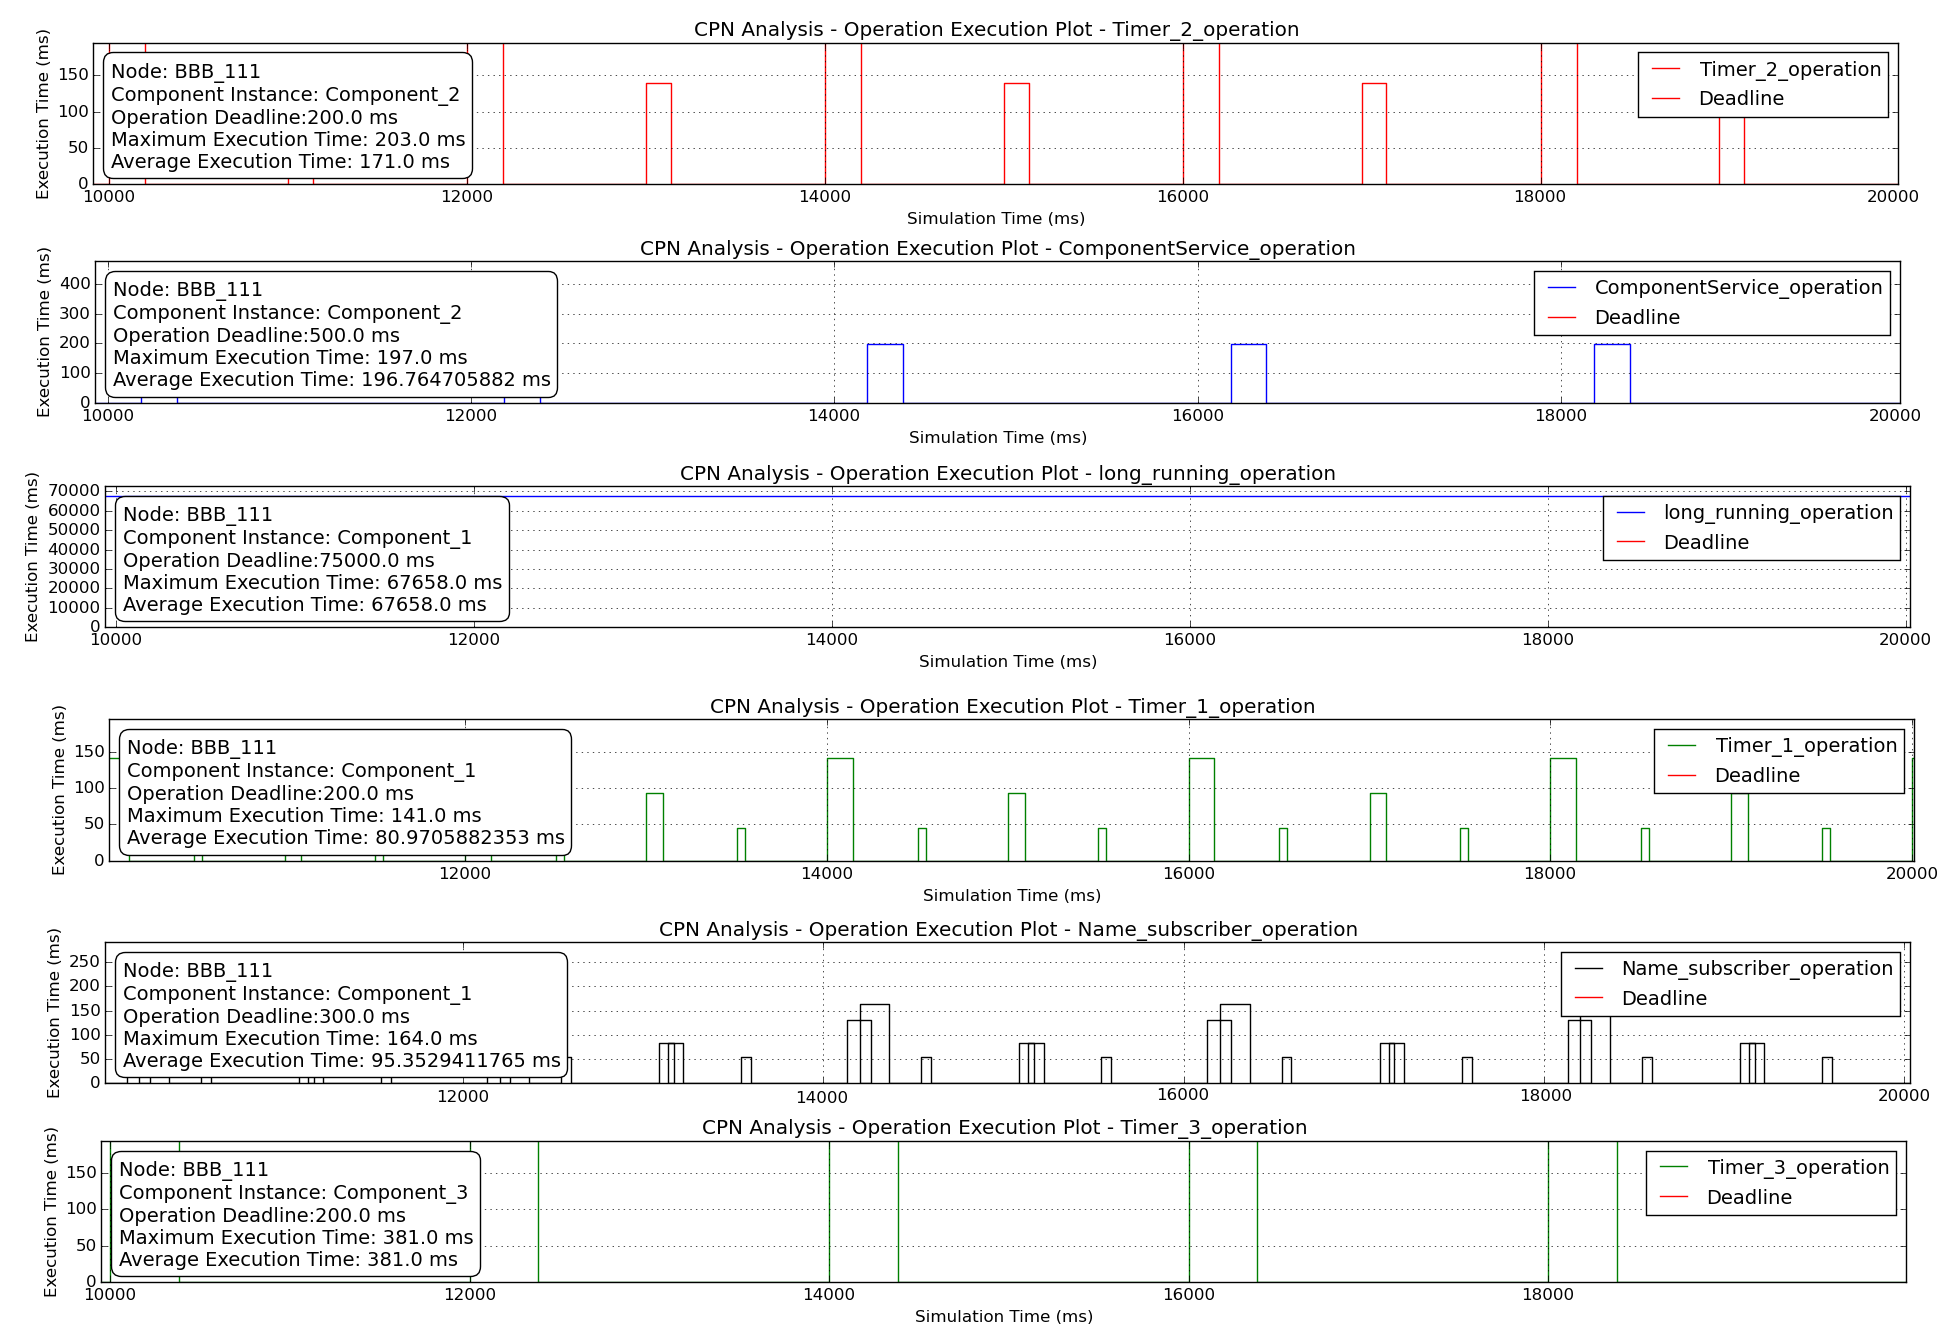
\includegraphics[width=\textwidth]{three-components-lro-cpn}
	\caption{Long Running Operations -- CPN Analysis Estimates. The CPN receives pure execution times of all operations in the component assembly from which a composed analysis is performed. The WCET plot is the representative worst-case execution trace obtained from state space analysis.}
	\label{fig:three-components-lro-cpn}
\end{figure*}

\subsection{Long-Running Operations}

Our ROSMOD component model implements a non-preemptive component operation scheduling scheme. A component operation that is in the queue, regardless of its priority, must wait for the currently executing operation to run to completion. This is a strict rule for operation scheduling and does not work best in all system designs e.g. in a long-running computation-intensive application, rejuvenating the executing operation periodically and restarting it at a previous checkpoint increases the likelihood of successfully completing the application execution. In applications executing long-running artificial intelligence (AI) search algorithms e.g. flight path planning algorithms, the computation should not hinder the prompt response requirements of highly critical operation requests such as sudden maneuver changes. Our ROSMOD component model does not support the \emph{cancellation} of long-running operations to service other highly critical operations waiting in the queue. With a few minor modifications to our scheduling schemes, long running operations can, however, be suspended if a higher priority waiting operation requires service. With these additions, we are able to model and analyze component-based systems that support long-running operations, with checkpoints, enabling the novel integration of artificial intelligence-type algorithms into our design and analysis framework. 

\subsubsection{Challenges}

One of the primary challenges here is to identify the semantics of a long-running component operation i.e. the scenarios under which the component operations scheduler suspends a cooperating long-running operation in favor of some other operation waiting in the queue. If a long-running computation is modeled as a sequence of execution steps with bounded checkpoints, then the operation would execute one step at a time and suspend at such checkpoints if necessary. An important challenge here is accurately identifying the priority difference between the long-running operation and the waiting operation. If the long-running operation is one checkpoint away from completion e.g. 100-200 ms of execution time, then strictly following our suspension rules would not be the most prudent choice since this operation is almost complete. However, if the waiting operation is a critical one, then regardless of the state of the long-running operation, the executing operation must be suspended.

\subsubsection{Implementation and Results}

In each long-running operation, we, therefore, include a synchronous \emph{checkpoint step}, as shown in Figure \ref{fig:lro-semantics}. The only assumption we make about this long-running operation is the periodicity of these checkpoint steps i.e. we know how frequently a new checkpoint is reached and we assume that the search algorithm used by the long-running operation is capable of reaching a safe state (the checkpoint) before suspending itself if required. If a higher priority operation is ready and waiting in the queue, the long-running operation runs till the next checkpoint is reached, then suspends. The higher priority operation is then processed. Figure \ref{fig:three-components-lro-rosmod} shows the \emph{Software Model} for a component assembly with long running operations.

The assembly consists of three components. Components \emph{Component\_1} and \emph{Component\_2} periodically publish on the \emph{ComponentName} message. \emph{Component\_3} periodically queries the server in \emph{Component\_2}. During these interactions, \emph{Component\_1} is performing a long running operation; the duration  of this operation is several times larger than the average execution time of all other operations. Figure \ref{fig:three-components-lro} shows the execution time plot of this scenario, as measured on our testbed. Figure \ref{fig:three-components-lro-cpn} shows our CPN analysis results for the same assembly. The plots represent the execution times of the various operation in the component assembly. As described in Section \ref{sec:ROSMOD}, execution time refers to the duration of time taken for an operation to be marked as 'complete' once it is enqueued on the component message queue. This explains the intersections in the plots for \emph{Name\_Subscriber\_operation} in \emph{Component\_1} as this is a subscriber port receiving messages on a same topic from two different publishers, in \emph{Component\_1} and \emph{Component\_2}. Secondly, it can be noted that the CPN predictions for \emph{Timer\_3\_operation} show no variation between the worst-case execution time and the average-case execution time (381.0 ms). This is because Component\_3 is not collocated with any other component and executing alone. Thus, the operation is not affected by any scheduling non-determinism or context switching delays. 
 
This exposes the conservative nature of the analysis. The Colored Petri net is an abstraction of the real execution behavior and makes several simplifications in order to obtain tractable analysis. Even still, there are analysis cases where the model is unable to perform as desired. For instance, the operating system (OS) scheduler uses a fixed-priority preemptive scheme with Round-Robin conflict resolution i.e. when two equal-priority threads are ready to execute, one is chosen at random and subsequently, Round-Robin scheduling is enforced. In the analysis, when we increase the number of equal-priority component threads, the state space of the analysis will explode since there are \emph{n!} possible thread execution orderings for \emph{n} equal priority threads executing on a device. The results of such an analysis may require searching a very large state space and may also cause a gross over-estimation of the execution times due to a single bad execution trace. This is a consequence of the simplified nature of the analysis, specifically the chosen OS scheduling model and the usage of worst-case execution times instead of other probabilistic methods. However, for strict safety-critical real-time systems that advocate predictable, deterministic behaviors, our analysis is still relevant. 
 
 \vspace{-0.1in}

%This means that the real deployment of the application threads \emph{never} exceeds the predicted worst-case execution times. Such results will validate the predicted timing properties of the system and ensure that the CPN analysis is useful and reliable.  


\section{Future Work}
\label{sec:Future-Work}

All of the results presented in this paper make an important assumption about the network -- the network resources available to each component is much larger than the requirements of the application i.e. there is no buffering delays on the network queues when components periodically produce data. We are currently working on integrating Network Calculus-based analysis methods \cite{ISIS_F6_CYPHY:14} into our CPN analysis for a more accurate profile of the analyzed application. This way, we can also model the system network profile (available bandwidth as a function of time) and realize the application data production profile, accounting for network delays caused by buffering. 

\section{Conclusions}
\label{sec:Conclusions}

In this paper, we have presented experimental validation for our Colored Petri net-based timing analysis methods for component-based distributed real-time systems. The validation covers a variety of component assemblies, interaction patterns and concepts, including publish subscribe-style messaging, client server-style querying, time-triggered interactions and long running operations. The results show close but conservative estimates from state space analysis and validate the utility of our tools and methods. 

\textbf{Acknowledgments:} The DARPA System F6 Program and the National
Science Foundation (CNS-1035655) supported
this work. Any opinions, findings, and conclusions or recommendations expressed
in this material are those of the authors and do not reflect the views of
DARPA or NSF. 
% \vspace{-0.1in}
\balance
\begin{spacing}{0.88}
\bibliographystyle{IEEEtran}
\bibliography{dissertation}
\end{spacing}

\end{document}
